\chapter{Power Minimizing Trees in Ad-hoc Wireless Networks}\label{chap:wanet}

A wireless ad-hoc network (WANET) is a collection of two or more devices with wireless communication and networking capabilities.
Broadly speaking, there are two models of wireless networks: single-hop and multi-hop.
The single-hop model is based on the cellular network model that provides one-hop wireless connectivity between mobile hosts and static nodes known as base stations \cite{clementi01}.
This network type relies on a fixed backbone infrastructure that interconnects all base stations by wired links.
Unlike cellular and wired networks, WANETs depend on neither a wired infrastructure nor pre-determined interconnectivity, and are thus a decentralized type of wireless network.

The set of uniform wireless communication devices with fixed locations are connected via wireless links depending on 
distance between the nodes, their transmission power, error control scheme, background noise and interference.
Each device is equipped with an omnidirectional antenna with a communication range schematically illustrated in Fig.~\ref{fig:omni}.
Hence, a signal reaches all nodes within the communication range of its sender.
This range is determined by the power assigned to the sender, and this power can be adjusted over time.
The power necessary for relaying a signal to multiple devices is the maximum rather than the sum of the powers necessary to reach all intended receivers.
This feature is referred to as the \emph{wireless advantage} \cite{wieselthier00}.
Each device works as a transceiver, which means that it can both transmit and receive a signal.

\begin{figure}[htb!]
    \centering
    \begin{subfigure}[b]{0.35\textwidth}
        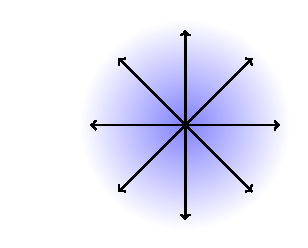
\includegraphics{figurer/omni-top.eps}
        \caption{Top view}
        \label{fig:omni-top}
    \end{subfigure}
    \begin{subfigure}[b]{0.55\textwidth}
        
\includegraphics{figurer/omni-side.eps}
        \caption{Side view}
        \label{fig:omni-side}
    \end{subfigure}
  \caption{Omnidirectional antenna}
	\label{fig:omni}
\end{figure}

The absence of infrastructure implies their quick deployment and simple configuration.
The recent years have witnessed an increasing interest in WANETs, motivated by numerous both civil and military applications and by the continual progression in wireless technologies.
Digital battlefield, disaster management, luggage handling in airports, 
context aware computing and mobile commerce are examples of the growing list of potential applications of WANETs \cite{younis06}.

%Fig. \ref{fig:communication} depicts different types of communication in wireless networks.
Consider a group of devices and a specific sender that initiates a signal transmission. 
A \emph{unicast} means that there is a single recipient.
Whenever the recipients are all the remaining devices within the group, we talk about a \emph{broadcast}.
Finally, a \emph{multicast} means that only some of the devices must receive the message. 
The remaining ones do not have to, but they can serve as intermediate devices forwarding the signal.

The wireless devices should be able to detect the presence of other such devices and to perform the necessary initialization to allow information sharing.
Since the devices can take different forms, their computation, storage and communication capabilities and battery capacity vary tremendously \cite{toh01}.
The wireless devices are typically heavily energy constrained due to the use of batteries as their energy source.
Energy conservation in WANETs is therefore a plentifully pursued research topic.
Most of the energy is spent on signal transmission \cite{halgamuge09}, 
and so it is desirable to design energy efficient transmission protocols that also satisfy certain requirements imposed on a WANET.

Various levels of connectivity are required on WANETs.
However, from a practical point of view, a topology which is ``too connected'' would often cause communication interference to occur even between nodes that are far apart.
Theoretical as well as practical experimental results suggest that the communication graph in WANETs should be as sparse as possible while preserving connectivity \cite{blough02}.

Models considered for WANETs are usually deterministic, that is, they assume that the nodes are fully reliable. 
In reality, the nodes are devices that may be subject to temporary or permanent failure due to technical damage or battery draining.
This fact leads to considering \emph{probabilistic} models whose aim is to capture the real world more plausibly by taking into account the uncertain character of nodes' availability.
Besides minimizing the power consumptions of the network, it is also required to guarantee a certain level of reliability over the whole network.

\section{Wireless Sensor Networks}

A related paradigm to WANET are Wireless Sensor Networks (WSN) which attracted a wide range of disciplines where close interactions with the physical environment are essential.
WSNs consists of tiny sensor nodes, which act as both data generators and network relays \cite{akyildiz10}.
Each node act as a sensor, a microprocessor, and a transceiver.
Sensor nodes have usually a fixed position and are powered by batteries.
Data measured  by sensors are transmitted via wireless communication links.

There are countless of sensor types, including seismic, electromagnetic, and acoustic, suggesting a broad area of practical application areas such as 
military, environmental, health, home, and industrial applications.

Multiple sensors are typically integrated into higher-level topologies varying in complexity.
These topologies can be divided into flat and hierarchical architecture \cite{mcgrath13}.
In a flat (peer to peer) architecture, every node has the same computational and communication capabilities.
In a hierarchical architecture, simple sensor nodes operate in close proximity to their respective \emph{cluster heads},
which possess more processing capacity than ordinary sensor nodes do.

WSNs are often built using one of the following configurations \cite{mcgrath13}:

\begin{itemize}
\item \emph{Point to point topology.} Links two endpoints either permanently or with the possibility of switching.
\item \emph{Bus topology.} Each node is connected to a shared communication bus, in which a signal is transmitted in both directions. 
\item \emph{Linear topology.} Two way link between one node and the next one, with two terminating nodes.
\item \emph{Ring topology.} A networks set up in a circular fashion is similar to linear topology, but does not contain the terminating nodes.
\item \emph{Star topology.} Consists of a single central node such as hub or a switch to which every node in the network is connected. 
An intelligent central node is required as all data traffic flows through it.
This topology is one of the most common WSN topologies.
\item \emph{Tree topology.} A hierarchy of nodes where in the highest level of the hierarchy is a single root node connected to one or many nodes in the level below.
The processing and power requirements in nodes increase as the data moves from the branches towards to root node.
\item \emph{Mesh topology.} Nodes disseminate their own data and also act as relays to propagate the data from other nodes.
The mesh topology can be partially connected  or fully connected (where there is a connection between every two nodes).
\end{itemize}
There is a need to reduce energy consumption so as to enhance the performance of the network in terms of lifetime, and a selection of suitable topology is therefore crucial.
Grid topology has been found energy efficient in theoretical comparison \cite{sharma13}, however, this may vary according to specific applications.
\section{Combinatorial optimization problems motivated by WANETs}

As indicated above, energy conservation is a crucial requirement in the design of WANETs. 
Combinatorial optimization is endowed with methods suitable for this task. 
It is necessary to introduce a formal network model in order to apply suitable mathematical tools.

\subsection{Network Model}

A WANET is modeled by a complete graph $G=(V,E)$, and a function $p:E\mapsto \mathbb{R}^+$.
The wireless devices are represented by nodes in $V$. 
As no power limit is imposed on the nodes, a transmission can be established between any two nodes, and thus $G$ is complete.
The function $p$ indicates the power requirement for sending a signal along a certain edge.
This requirement depends on distance and environmental properties, and is given by  $p_{ij}=\kappa d_{ij}^\alpha$, 
where $d_{ij}$ is the Euclidean distance between the devices represented by nodes $i$ and $j$, $\alpha$ is the constant environmentally dependent factor typically valued between 2 and 4,
and $\kappa\geq 0$ is the transmission quality parameter. 
Since the value of $\kappa$ does not affect the optimal solution, it is often assumed to be 1.
The transmission range of a node $i$ depends on the power supply $P_i$ assigned to it.
The overall power assignment to individual nodes induces a directed transmission graph (see the example in Fig.~\ref{fig:transgraph}). 
On the other hand, for a given transmission graph, the power assignment to a node corresponds to its longest outgoing arc.
\begin{figure}[htb!]
  \centering
  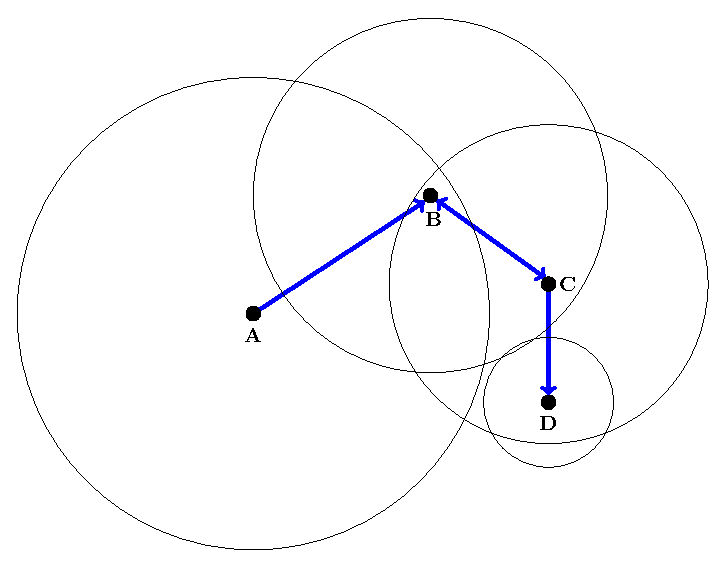
\includegraphics[scale=.8]{figurer/tran-graph.eps}
  \caption{Power assignment to nodes (circles)  and corresponding induced transmission graph (blue arrows)}
  \label{fig:transgraph}
\end{figure}
It is usually assumed that nodes are distributed in a Euclidean space, although there are multiple results on variants where general input graphs are considered.
In the following combinatorial problems motivated by WANETs, the task is to assign powers to individual nodes while satisfying certain criteria so that the overall power is minimized.
The total power is expressed by an objective function varying among the problems.

\subsubsection{Multicasting}

%Additional assumption of the existence of nodes that never initiate any transmission, nor they have to receive any signal, is a natural extension of all the problems described above.
%These nodes can act as intermediate nodes relaying the signal, if improves the respective objective function value.
In certain situations, some of the wireless nodes never initiate any transmission, nor they have to receive any signal.
Including them in the network may lead to a more efficient communication.
Assumption of the existence of these nodes is often studied as an extension of the problems described in the sections below.
In addition to the graph $G$ and the power requirement vector $p$, the set of nodes $D\subseteq V$, called \emph{destinations}, is also a part of the input.
Nodes in $V\setminus D$ are referred to as \emph{non-destinations}.
The inclusion of non-destination nodes resembles the generalization of MST leading to the \textsc{Minimum Steiner tree} problem.
In WANET scenarios, the presence of such nodes is often referred to as a \emph{multicast} version.

\subsection{Minimum Energy Broadcast}

The \textsc{Minimum Energy Broadcast} (MEB) problem consists of a node set $V$ and a specified source $s\in V$, that is supposed to initiate a transmission.
All the remaining nodes must receive the signal via communication links induced by power assignment to the nodes.
\begin{problem}\label{prob:meb1}
Given a directed graph $G=(V,A)$, a source $s\in V$, and power requirements $p$, find a power vector $(P_1,P_2,\dots,P_n)\in\mathbb{R}^n$ of minimum component sum such that
there exists a path from $s$ to each $t\in V\setminus\{s\}$ in $G^P(V,A^P)$, where $A^P=\{(i,j)\in A: p_{ij}\leq P_i\}$.
\end{problem}
For two distinct nodes $u$ and $v$  in $G$, the optimal solutions to MEB on the input $(G,u,p)$ and $(G,v,p)$ may differ.
An optimal solution differs for different transmission sources.
Hence, the nodes must by endowed with a mechanism that allows them to adjust their power level for a corresponding transmission session.
This places demands on the computational capacity and technological solution of the nodes.
The advantage of this concept lays in the optimality of each broadcast session.

The directed graph induced by power assignments as defined in Problem~\ref{prob:meb1} is not necessarily an arborescence.
However, MEB could be stated slightly differently:
\begin{problem}\label{prob:meb2}
Given a directed graph $G=(V,A)$, a source $s\in V$, and power requirements $p$, find an arborescence $T$ spanning $G$ rooted at $s$ minimizing 
	$$\sum\limits_{i\in V}\max\limits_{j\in N^-_{T}(i)}p_{ij}.$$
%such that the sum of the weights of the heaviest outgoing arcs from all nodes is minimized.
\end{problem}

\begin{observation}
The optimal objective function value of a given instance is equal in Problem~\ref{prob:meb1} and~\ref{prob:meb2}.
\end{observation}

MEB has received a significant attention during the last two decades.
The problem has been introduced in \cite{wieselthier00}, where the authors suggest three greedy heuristic methods and an additional ``sweep'' operation aiming to remove unncecessary transmission:
\paragraph{MST algorithm.}
A MST is constructed, and subsequently the edges are oriented towards the leaves, starting from the source.
The last step is to assign power levels to each node $v$ according to the longest arc outgoing from $v$.
\paragraph{SPT algorithm.}
The shortest path tree (SPT) algorithm establishes a minimum-cost path from the source node to every other node.
The broadcast tree consists of superpositions of these unicast paths.
\paragraph{BIP algorithm.}
The Broadcast Incremental Power (BIP) algorithm resembles Prim's algorithm for MST.
BIP gradually constructs a broadcast tree as follows:
\begin{itemize}
\item Initially, the tree $T$ contains only the source $s$, and all nodes have zero power assignment.
\item While there are some nodes outside of $T$
\begin{itemize}
	\item Find a node $v$ not already in $T$ whose addition to $T$ results in a minimum increase of power assignments of some node $u$ already in $T$, and add $v$ to $T$.
	\item Increase the power assignment of $u$ so that $v$ is reached.
\end{itemize}
\end{itemize}
\paragraph{The sweep operation.}
Sweep can be applied after a solution $T$ is constructed by one of the methods above.
It can be called iteratively to its own input to further improve the solution.
Non-leaf nodes in $T$ are inspected one by one, and if for some node $v$ there exists $u\in N^-(v)$ such that power assignment of $v$ is sufficient to reach all nodes in $N^-(u)$, 
then the transmission of $u$ is eliminated.

\subsubsection{Problem complexity and approximability}

NP-hardness results for both general and geometric MEB are provided in \cite{cagalj02} by reduction from \textsc{Set Cover} and \textsc{Planar 3-SAT}, respectively.
In the former case, the network topology is represented by a generic graph with arbitrary weights, whereas in the latter a Euclidean distance is considered.
The special case where $\alpha=1$, i.e., where the edge weights correspond to distances between the endpoints belongs to the complexity class $P$.
An optimal solution is determined trivially by assigning minimum power sufficient to reach all nodes in a single hop, regardless of the nodes' arrangement.

The first analytical study of the three methods proposed in \cite{wieselthier00} is given in \cite{wan02}, where the authors provide quantitative characterization in terms of approximation ratios.
It has been showed that the approximation ratio of MST and BIP lies in the interval $\left[6,12\right]$ and $\left[13/3,12\right]$, respectively.
The approximation ratio of SPT is proved to be at least $n/2$.
These results were gradually improved in several works. 
The upper bound of the MST algorithm was improved to 6 in \cite{ambuhl05}, which closes the gap. %, and thus proves its optimality.
This upper bound is valid for BIP as well, due to a lemma in \cite{wan02},
which says that for Euclidean instances of MEB, the objective function value of a solution obtained by BIP is at most the weight of a MST for this instance.
The lower bound on the approximation ratio of BIP was strengthened to 4.598 in \cite{bauer09}. 
This work also devises an implementation of BIP with improved time complexity $\mathcal{O}(|V|^2)$.

\subsubsection{Problem variants}

As an extension of MEB, the introduction of non-destinations leads to the Minimum Energy Multicast (MEM) problem, introduced along with MEB in \cite{wieselthier00}.
It is easy to see that MEM is NP-hard due to the fact that MEB is a special case where $D=V$. %, or by reducing the \textsc{Minimum Steiner tree} problem to it.

A variant of MEB, assuming that there are $k$ adjustable power levels $w_{i,1},w_{i,2},\dots w_{i,k}$ at each node $i$ is studied in \cite{liang02}.
This problem remains NP-hard which is proved by reducing \textsc{3-CNF-SAT} to it.
In addition, \cite{liang02} contains an approximation algorithm for this version of MEB with a performance guarantee $\mathcal{O}(n^\epsilon)$ and 
time complexity $\mathcal{O}((k+1)^{\frac{1}{\epsilon}} n^{\frac{3}{\epsilon}})$ for $\epsilon\in \left(0,1\right]$.
Another restriction considered in \cite{liang02} is that each node has the same adjustable power levels, i.e., $w_{i,l}=w_{j,l}$ for $1\leq l\leq k$ and $1\leq i,j\leq n$.
For this problem, another approximation algorithm, which delivers a solution within $\mathcal{O}(\log^3 n)$ times the optimum is devised.

Probabilistic MEB, where a node reliability is considered, has also been investigated.
Three ILP formulations of probabilistic MEB together with suitable solving methods are developed in \cite{montemanni08}.
Another study of ILP formulations and suitable valid inequalities is pursued by \cite{barta10}.

A restriction of node locations can be imposed.
One example is a random grid network, where nodes are chosen independently and randomly from points of a $\sqrt{n}\times\sqrt{n}$ square grid in the plane.
The probability distribution of existence of a node can be non-uniform.
A lower bound on the optimal objective function value is proved in \cite{calamoneri08} together with a near optimal construction method.
The 6-approximation of MST turns out to be too pessimistic for instances with restricted node locations which represent the real-life instances more closely.
The authors of~\cite{flammini07} argue that the approximation ratio of MST the algorithm can be considered close to 4 for practical instances.

\subsubsection{ILP models}

Integer linear programs for MEB are studied in various works.
Three ILP formulations are proposed in \cite{das03}.
The first formulation assumes exactly one transmission from the source $s$, and at most one transmission from each node in $V\setminus\{s\}$.
This formulation operates with order of transmissions which helps to establish connectivity of the resulting solution.
Power assignments are straightforwardly modeled by one continuous variable for each node, leading to an objective function minimizing their sum.

The same objective function is used in the second formulation.
In contrast, the second formulation allows at least one transmission from the source, and an arbitrary number of transmissions from the other nodes.
The necessary subtour elimination is achieved by additional ``sequencing variables'', proposed for the \textsc{Traveling Salesman Problem}.

The last formulation is built upon a single-commodity network flow model, and its interpretation follows from the second formulation.

A similar formulation is proposed in \cite{yuan05}, where the continuous power variables for each node are replaced by binary variables $y_{ij}$ for each pair $(i,j)$ of nodes,
attaining the value 1 if and only if the power of node $i$ equals $p_{ij}$.
Connectivity is achieved by multi-commodity flow variables and associated flow conservation constraints.

The authors of~\cite{haugland11} provide a formal proof that using binary power variables instead of continuous ones leads to a stronger formulation,
which can be further strengthened by introducing the multi-commodity flow variables.

Yet another network flow model formulation along with efficient solution techniques utilizes a fast solution of a combinatorial relaxation of the model \cite{min06}.

\subsubsection{Planarity of an optimal solution}

Alternatively to Problem~\ref{prob:meb1} and \ref{prob:meb2}, a MEB instance can be specified by $G=(V,E)$, $s\in $V, and coordinates $\left[x_v,y_v\right]$ for each node $v\in V$.
%We recall from Section \ref{sect:back:graph} that an embedding of a graph in a plane assigns coordinates to nodes in a Euclidean plane.
These coordinates implicitly imply distance $d_{ij}$ between every two nodes $i$ and $j$.

We address the question whether an optimal solution to various MEB instances has a planar embedding.
To the best of our knowledge, the available literature does not provide results on this topic.
The unpublished findings presented below are based on the assumption that a feasible solution to MEB is a tree as stated by Prob.~\ref{prob:meb2}.

By inspecting a large number of instances and their optimal solution, the planarity of the optimum cannot be guaranteed in general, even though in the majority of cases, the optimum is indeed planar.
\begin{proposition}\label{prop:mebplan}
Consider nodes 4 nodes in an instance of MEB that form a convex quadrilateral $ABCD$.
If two non-adjacent sides of the quadrilateral are shorter than the shorter diagonal, then in an optimal solution, edges with both endpoints in $ABCD$ do not cross each other.
\end{proposition}
\begin{proof}
Consider the quadrilateral as depicted in Fig~\ref{fig:quad}. 
\begin{figure}[htb!]
  \centering
  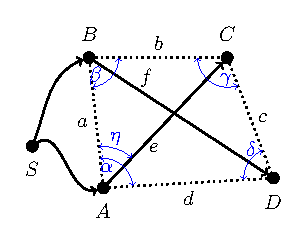
\includegraphics[scale=1.4]{figurer/quadrilat.eps}
  \caption{Four nodes forming a convex quadrilateral}
  \label{fig:quad}
\end{figure}
Without loss of generality, let $d_{AC}\leq d_{BD}$, $d_{AB}\leq d_{AC}\leq d_{BC}$ and $d_{CD}\leq d_{AC}\leq d_{AD}$.
By the law of cosine, we have that 
$$
\cos{\beta}=\frac{d^2_{AB} + d^2_{BC} - d^2_{AC}}{2d_{AB}d_{BC}} \text{~~~ and ~~~}\cos{\delta}=\frac{d^2_{CD} + d^2_{AD} - d^2_{AC}}{2d_{CD}d_{AD}}.
$$
Both numerators are positive, both $\beta$ and $\delta$ are acute, which immediately implies that $\alpha $ and $\gamma$ are obtuse.

Let $T=(V,A_T)$ be an optimal solution to the given instance.
If $(A,C)\in A_T$ and $(B,D)\in A_T$, $(A,C)$ covers $B$ due to the wireless advantage, and $(B,D)$ covers $C$ because $\gamma$ is obtuse.
Then, by replacing $(A,C)$ with $(A,B)$ we get rid of the crossing and all four nodes are covered.
If $(A,C)\in A_T$ and $(D,B)\in A_T$, $(D,B)$ covers both $A$ and $C$ as $\alpha$ and $\gamma$ are obtuse, thus $(A,C)$ can be removed without disconnecting the solution.
The remaining cases are symmetric.
\end{proof}
If the condition that the shorter sides must not be adjacent is not met in Prop.~\ref{prop:mebplan}, a crossing may occur, as example in Fig.~\ref{fig:mebnonplan} demonstrates.
\begin{figure}[htb!]
  \centering
  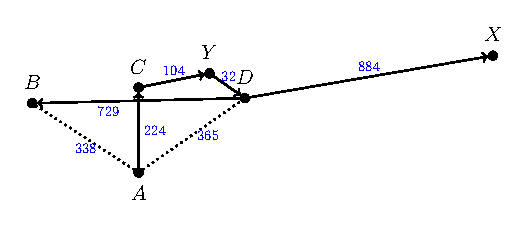
\includegraphics[scale=1.4]{figurer/mebnonplanar.eps}
  \caption{A unique optimal solution with crossing to a Euclidean instance of  MEB with source in node $A$.
  The blue edge weights correspond to the power requirements between two nodes. 
  The nodes have coordinates $A=[75,63]$, $B=[50,77]$, $C=[49,63]$, $D=[50,50]$, $X=[45,22]$ and $Y=[47,55]$.
  For convenient display, lengths of edges in the figure are not proportional.}
  \label{fig:mebnonplan}
\end{figure}

\subsection{Range Assignment Problem}

In the \textsc{Range Assignment Problem} (RAP), the task is to minimize the total power consumed under the constraint 
that adequate power is provided to the nodes to ensure a strong connectivity of the graph.
Formally, the problem is stated as follows:
%Therefore, only one broadcast tree is stored which is common for all possible sources.
\begin{problem}
Given a directed graph $G=(V,A)$ and power requirements $p$, find a power vector $(P_1,P_2,\dots,P_n)\in\mathbb{R}^n$ of minimum sum such that the induced graph $G^P=(V,A^P)$ is strongly connected, 
where $A^P=\{(i,j)\in A: p_{ij}\leq P_i\}$.
%every where $E^P=\{(i,j)\in E: p_{ij}\leq P_i\wedge p_{ij}\leq P_j\}$.
\end{problem}

An obvious advantage of RAP over MEB is that a single transmission graph is constructed in RAP regardless of the source node.
However, this can lead to solutions optimal with respect to RAP, but for certain sources initiating the transmission, the solution can be too expensive.
Sect.~\ref{sec:sbt} describes a problem with a more complicated objective function that combines advantages of both RAP and MEB.

\subsubsection{Problem complexity and approximability}

In \cite{kirousis00}, it is shown that for instances consisting of collinear points, there exists an algorithm that solves the problem to optimality in $\mathcal{O}(n^4)$.
The authors further prove by reduction from \textsc{Vertex Cover} that RAP in 3-dimensional Euclidean space is NP-hard for any value of $\alpha$,
and that there exists a $\mathcal{O}(n^2)$ time 2-approximation algorithm based on finding MST.
The results are strengthened in \cite{clementi99}, where it is proved that RAP is NP-hard for instances in a 2-dimensional Euclidean space for any $\alpha$, 
and that for 3-dimensional space, the problem is APX-complete, thus does not admit a PTAS unless P$=$NP.
Let us recall that unlike RAP, for $\alpha=1$, when the power requirements equal the distances, MEB  is solvable in polynomial time.
An approximation algorithm improving the performance guarantee approaching 1.69 is presented in~\cite{calinescu02}.
For the case $\alpha=1$, there exists an approximation algorithm with performance guarantee 1.5~\cite{ambuhl03}.
A recent work \cite{carmi15} achieves an exact algorithm for the 1-dimensional problem that runs in $\mathcal{O}(n^2)$.

\subsubsection{Problem variants}

A further constraint requires that diameter of the transmission graph has to be at most some constant value $h$.
On a family of instances limiting the proximity of two nodes, this variant of RAP is in APX \cite{clementi01b}.
The 1-dimensional problem with restricted diameter (number of hops) has been studied in \cite{clementi03}, where the authors introduce an exact algorithm that runs in $\mathcal{O}(hn^2)$.

Another modifications imposes symmetric communication links.
This version is often found in the literature under the abbreviation SRAP.
In a generalized version, weakly symmetric RAP (WSRAP), the symmetry requirement applies only to a pre-defined subset of edges.
Other edges which are not essential for connectivity are allowed to be unidirectional.
The motivation for studying WSRA stems from the observation that what is really important in the design of WANETs and WSNs is the existence of a connected backbone of symmetric edges \cite{santi05}.
Imposing symmetry does not change the complexity of the problem, which remains NP-hard in two and three-dimensional networks \cite{blough02}.

The abbreviation SRAP is sometimes used for the Steiner RAP, where there is a predefined subset $D\subseteq V$ of destination nodes that are required to be included in a solution.
The remaining Steiner nodes take part in the solution only if their presence reduces the objective function value.
If not stated otherwise, SRAP in this work refers to the Symmetric RAP.

\subsubsection{ILP models}

An ILP model with an exponential number of constraints along with a cutting plane method solving it is presented in \cite{althaus03}.
A model based on network flows with polynomial number of constraints is introduced in \cite{das04}.
Although this work concerns SRAP with directional antennas, their model can be adapted to the more common version with omnidirectional antennas.
For modelling the power assignments, this model uses continuous power variables.
By replacing them with binary ones and a corresponding adjustments in the model \cite{montemanni05, haugland11}, it is possible to achieve a stronger formulation.
Even stronger model uses multi-commodity network flow variables \cite{haugland11}. 
These strength results are analogous to those regarding MEB.
Yet stronger formulation is obtained by using a multi-tree model \cite{haugland11}. 
The authors employ binary variables indicating whether or not an arc $(i,j)$ is in the arborescence rooted at $t\in D$.
This model is thus applicable for the Steiner RAP.

\subsection{Shared Broadcast Trees}\label{sec:sbt}

The idea of broadcasting using a single broadcast tree was first investigated in \cite{papadimitriou06}.
The Shared Broadcast Tree (SBT) problem in the form presented here was pursued in \cite{yuan12}, where the authors present an ILP model along with a suitable solving method.

A feasible solution to the SBT problem is any (undirected) spanning tree.
This concept is motivated by the intention of incorporating the frequency of use of each node for different broadcast sessions.
Every node can transmit a signal, but some are actively transmitting more often than others.
We assume that a node acts as a source with a uniform probability. 
A leave $l$ transmits a signal only when $l$ is the source, other intermediate nodes transmit more often as they also relay signals initiated in other nodes.

Observe that a forwarding node that received a signal does not have to send it back to the node from which the signal was received.
If the signal was received in a node $i$ from its most distant neighbor node $i_1$, it has to be forwarded to nodes that have not received it yet along the link to the second most distant node $i_2$.
Due to the wireless advantage, all other neighbor nodes closer than $i_2$ receive it as well.
Conversely, if the signal was received by $i$ from a neighbor node different from its most distant neighbor $i_1$, node $i$ has to forward it to $i_1$. 
It is therefore evident that $i$ does not have to always transmit with the power corresponding to the most distant neighbour.
It transmits either with power level $p_{ii_2}$, if the signal came from the most distant node $i_1$, or with power level $p_{ii_2}$, otherwise.
The situation is depicted in Fig~\ref{fig:objexp}.
\begin{figure}[htb!]
  \centering
  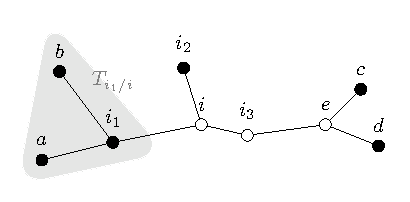
\includegraphics[scale=1.4]{figurer/objexp.eps}
  \caption{Example instance explaining power levels necessary for transmitting a signal from different sources}
  \label{fig:objexp}
\end{figure}

Consider an edge $\{i,j\}$ in a solution $T$ to SBT.
Let $T_{i/j}$ denote the subtree of $T$ consisting of nodes whose path to $j$ contains $(i,j)$. 
A node $i$ in $T$ contributes to the objective function by the expression $c_T(i)$ as follows:
\begin{equation}\label{eq:sbtnodecontr}
c_T(i)=|T_{i_1/i}|p_{ii_2} + |T\setminus T_{i_1/i}|p_{ii_1}.
\end{equation}
We can also regard $c_T(i)$ as a weighted arithmetic mean of $i$'s power levels, with weights corresponding to the number of nodes whose signal is transmitted using the corresponding power level.
The objective function is to minimize overall nodes' contributions, that is,
\begin{equation}
c(T)=\sum\limits_{i\in V}c_T(i).
\label{eq:sbtcost}
\end{equation}
The problem under study is thus defined as follows:
\begin{problem}
Find a tree $T\subseteq G$ spanning $D$ minimizing \eqref{eq:sbtcost}.
\end{problem}

\emph{Remark:} The requirement that a solution must be a tree is necessary due to the nature of the objective function.

Like in MEB, an optimal solution to SBT does not guarantee a planarity of the resulting tree, although vast majority of instances are planar. 
As an example of non-planar optimum we state the instance on five nodes depicted in Fig~\ref{fig:sbtnonplanar}.
\begin{figure}[htb!]
  \centering
  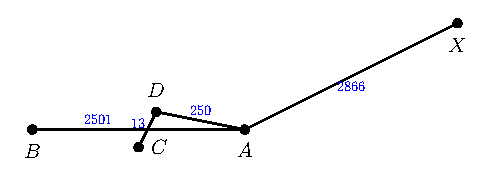
\includegraphics[scale=1.4]{figurer/sbtnonplanar.eps}
  \caption{A unique optimal solution with crossing to an instance of SBT with objective function value 19904. 
  If the arc $(DC)$ is forbidden, the optimal solution becomes a star graph with objective function value 19917.
  The nodes have coordinates $A=[50,30]$, $B=[49,80]$, $C=[51,48]$, $D=[48,46]$ and $X=[5,1]$.}
  \label{fig:sbtnonplanar}
\end{figure}

The presence of Steiner nodes that are not required to be a part of the resulting tree leads to the Shared Multicast Tree (SMT).
Some preliminary results were published in Paper I~\cite{ivanova16}, which contains ILP model and a heuristic methods with local search improvements.
Further investigation of the ILP model and a more extensive experimental evaluation is given in Paper III.

In SMT, the objective function has to be adjusted accordingly. 
The contribution of a single node must reflect the fact that non-destination nodes do not initiate any transmission.
Let us define the function $\mu: G\mapsto \mathbb{N}^+_0$ that returns the number of destinations in a given graph $G$.
The contribution of one node in a solution $T$ to the resulting objective function given by Eq.~\ref{eq:sbtnodecontr} is in SMT changed to 
\begin{equation}\label{eq:smtnodecontr}
c_T(i)=\mu(T_{i_1/i})p_{ii_2} + \mu(T\setminus T_{i_1/i})p_{ii_1}.
\end{equation}
This objective function takes into account energy consumption by transmission only.
Available literature of multicast versions of MEB and RAP applies this energy model too, however, it is also possible to incorporate other,
less significant energy consumption sources as indicated by \cite{halgamuge09}.
As each node that participates in the solution poses an additional energy outlay $\epsilon$, the objective function~\ref{eq:sbtcost} would then become
\begin{equation}
c(T)=\epsilon|V_T|+\sum\limits_{i\in V}c_T(i),
\label{eq:smtcostB}
\end{equation}
if the energy expenses of each node are homogeneous. 

